\chapter{Theoretical Overview}

At the heart of particle physics is a quest to discover the fundamental building blocks of the universe, and how they interact with one another. Experimentally this is done by delving into smaller and smaller distance scales using particle colliders with greater energies and analysing the interactions that result. This relationship between small distances and high energies is at the heart of the field, as each increase of energy scale allows the investigation of the structure of matter at a smaller length scale. Throughout the history knowledge has been advanced through a combination of theoretical postulation using mathematical tools, and experimental searches. Particle physicists seek together to build a full description of the dynamics of the fundamental particles, and while they have discovered much, the picture is not complete yet. The current state of play is collectively known as the Standard Model (SM), and is a rigorously tested and widely accepted theory. However, whilst there are no disagreements, there are some gaps which hint at physics beyond, fuelling a new generation of experimentalists seeking answers to what lies behind.

\section{The Standard Model}

The Standard Model (SM) is the name given to the theories that successfully describes the known elementary particles and their fundamental interactions with respect to the strong, weak and electromagnetic forces.  These theories are formulated mathematically using Quantum Field Theory (QFT), in which particles are thought of as excitations of fields, and the dynamics of a given system are summarised in what is known as Lagrangian formalism. In this the Lagrangian L is the difference between kinetic energy T and potential energy V, $L = T - V$. In QFT it is usual to describe a system by the Lagrangian Field Density $\Lagr$, where L is obtained from $\Lagr$ by integrating over the spatial component $d^{3}x$.

In order to reflect the symmetries observed in nature, measurements of physical properties in the SM, and therefore the Lagrangian Density $\Lagr$, must be invariant under some set of transformations,

\begin{equation}
\psi \rightarrow e^{-i\alpha}\psi 
\label{GlobalTrans}
\end{equation}


where $\psi$ represents a spinor field. If $\alpha$ has no reliance on the space-time coordinate, we say this is a global symmetry. In order to describe the fundamental interactions it is necessary to use the special case where the transformations are \textit{local}, where $\alpha$ has a dependence on the space-time coordinate. The Standard Model describes such symmetries, a case we call gauge invariance, and is a special case of field theory known as Gauge Theory, where the transformations have the form, 


\begin{equation}
\psi(x) \rightarrow e^{-i\alpha(x)}\psi (x) 
\label{LocalTrans}
\end{equation}


It is clear that $\Lagr$ will not remain unchanged by such a transformation, as the dependence of $\alpha$ on $x$ means that the coordinate derivative $\partial_{\mu}$ introduces extra terms. In order to leave the Lagrangian unchanged a vector field is introduced $A_{\mu}$ that transforms under another local transformation to keep $\Lagr$ constant: 

\begin{equation}
A_{\mu} \rightarrow A_{mu} + \frac{1}{g} \partial_{\mu} \alpha(x)
\label{ATrans}
\end{equation}

Thus we can rewrite $\Lagr$ introducing the \textit{covariant derivative}, 
\begin{equation}
\Dev_{\mu} = \partial_{\mu} - igA_{\mu}. 
\end{equation}

This interaction between the spinor field and the vector field through this covariant derivative indicate the interactions of matter particles though the force carrying bosons. From Noether's Theorem, it is known that as a consequence of a symmetry in a dynamical system there is an associated physically conserved quantity\cite{Rolnick}. Just as the classical conservation laws pertaining to momentum and energy are given by the space-time translational symmetries in Classical Mechanics, for the electromagnetic force symmetries in Quantum Mechanics the electric charge is conserved. Analogously, there ought to be conserved "charges" for the strong and weak forces also. 
 
The set of possible transformations is described in the language of Group Theory, and thus we describe the SM as a non-Abelian Yang-Mills type gauge field theory based on the symmetry group $SU(3)_{C} \times SU(2)_{L} \times U(1)_{Y}$. As this group is a product the three individual elements are free to each have its own coupling constant, and these may differ. The strong interactions described by Quantum Chromodynamics (QCD) are represented by $SU(3)_{C}$, and the electromagnetic and weak interactions are represented together due to Electroweak Unification by the group $SU(2)_L \times U(1)_{Y}$. As of yet, the fourth fundamental force Gravity is not included in the Standard Model, but this is seen as of little consequence as gravitational forces are thought to have comparatively little effect on fundamental particles. 


There exist two main types of fundamental particle, which in order to distinguish we must address the concept of spin. 
\begin{description}
\item[Spin] \hfill \\
Spin is the name given to a property of elementary particles, corresponding to a type of angular momentum, although this differs from classical angular momentum. This is an intrinsic property and thus has a specific value for each particle type. It can be thought for massive particles as the angular momentum about the central point, but it is known that massless particles such as the photon carry spin also, so this analogy breaks down. The values of the spin quantum number s which describe the magnitude can take any half integer value $s=0, \frac{1}{2}, 1, \frac{3}{2}$, etc. In addition to magnitude we describe a particle as having spin \textit{up} (positive) when the spin is in the direction of the z-axis, and spin \textit{down} (negative) if the spin is against the direction of the z-axis. 

When the spin direction is in the direction of momentum of the particle, it is described as left-handed, and when it is against as right-handed. This handedness is integral to the way these particles behave, as we will see in the treatment of the weak force. 
\end{description}
All fundamental particles are divided into the spin-1/2 \textit{fermions} which are the building blocks for matter, and the force-mediating \textit{bosons} which must carry integer spin, usually spin-1. 
 

The fermions which make up all visible matter can be described in three families, or "generations", shown in Equation \ref{eqn:threefams}. Within each generation, there are two sets of particles, those on the left are the leptons, which interact by the weak and electromagnetic forces only, and those on the right are the quarks, which also interact by the strong force. In each generation, there are two quarks, which differ by electoral charge - one has +2/3 and the other -1/3 (in units of the electron charge \textit{e}), an electrically charged lepton and a neutral lepton called a neutrino which is either massless or very light. The three families then are organised in ascending order of mass. The first generation is therefore stable and all ordinary matter is constructed from it, whilst the second and third are liable to decay into particles of the first generation. In addition to each particle detailed here there exists a corresponding antiparticle due to a symmetry in charge and quantum numbers.  Each fermion can be described as a spinor field $\psi$ which describes a pair of complex fields, the left-handed ($\psi_{L}$)and right-handed ($\psi_{R}$) representations. 
 
\begin{equation}
\begin{bmatrix}
\nu_{e} & u \\
e & d \\
\end{bmatrix},
\begin{bmatrix}
\nu_{\mu} & c \\
\mu & s \\
\end{bmatrix},
\begin{bmatrix}
\nu_{\tau} & t \\
\tau & b\\
\end{bmatrix}
\label{eqn:threefams}
\end{equation}

The particles which mediate the forces are bosons, the photon $\gamma$ for the electromagnetic force, the 8 gluons $g_{i}$ for the strong force and the $W^{\pm}$ and Z bosons that carry the Weak force, all of which are spin-1 particles. The final particle of the SM is the Higgs Boson of spin-0, as yet undiscovered in experiment but expected from the theory, as we will see later. 

\subsection{Gauge Theory of Interactions}

Everything in our Universe interacts by way of gauge bosons mediating one of the four fundamental forces. Whilst the SM incorporates the electromagnetic, strong and weak forces, it as of yet has not been possible to describe the gravitational force in this way. 


\subsubsection{Quantum ElectroDynamics}

The fundamental electromagnetic force is studied in quantum field theory as Quaaludeantum Electrodynamics (QED), the oldest and simplest of the theories brought together to form the SM. The symmetry of QED is U(1) and this gives an associated conserved quantity, the electric charge Q. The electromagnetic force is carried by the massless boson, the photon, and affects only the charged fermions. The symmetry allows no self interaction of the photon. The fermion field $\psi_{q}$ with charge $q$ and mass $m_{q}$ with symmetries under the group of transformations $e^{-i\alpha(\stc)}$ gives rise to the Lagrangian in Equation \ref{eqn:QEDL}.
\begin{equation}
\Lagr_{QED} = \bar{\psi}_{q}(i \gamma^{\mu}\slashed{D}_{QED} - m_{q}) \psi_{q} - \frac{1}{4}F_{\mu \nu}F^{\mu \nu}
\label{eqn:QEDL}
\end{equation}

The kinetic term depends on the Field Strength Tensor F, 
\begin{equation}
F_{\mu \nu} (\stc) = \partial_{\mu} A_{\nu}(\stc) -   \partial_{\nu} A_{\mu}(\stc) 
\end{equation}

which incorporates the introduction of a gauge field $A_{\mu}$ which is transformed along with $\psi$ in the following way:

\begin{equation}
A_{\mu}(\stc) \rightarrow A_{\mu}(\stc) + \partial_{\mu} \alpha(\stc)
\label{AQED}
\end{equation}

The  covariant derivative, $\slashed{D}_{QED,\mu}$ is defined as in Equation \ref{eqn:QEDD} so as to maintain an invariance to local U(1) charge symmetry. 
\begin{equation}
\slashed{D}_{QED} = \partial_{\mu} + iqA_{\mu}
\label{eqn:QEDD}
\end{equation}


where q is described as the generator of the symmetry group and is analogous to electric charge. The strength of coupling of each force is described by the coupling constant, in this case governed by the constant e, the charge of an electron: $\alpha = \frac{e^{2}}{4\pi}$. This is more commonly known as the \textit{fine structure constant} and has been measured experimentally to a high degree of accuracy to have a value $\alpha = \sfrac{1}{137}$ \cite{qedalpha}. 

\subsubsection{QCD}

Quantum Chromodynamics (QCD) is the relevant quantum field theory that describes the dynamics of the strong force. The strong force of symmetry group $SU(3)_{C}$ has 8 massless gauge bosons known as the gluons, and a conserved quantity called colour charge, which has three types called $q_{i} i=1,2,3$. The name "colour" is not meant to imply a connection to visual colour, merely an analogy between the three types and the primary colours red, blue and green. Only particles which carry colour charge are affected - the quarks have colour, while leptons do not. Unlike the photon in electromagnetism, the gluons that mediate the force carry the charge also, leading to the self-interactions that govern the behaviour of QCD. 

A quark carries one "colour" $q_{i}$, taking one of the three possible values, and an analogous antiquark carries one "anti-colour". On the other hand, gluons carry both a colour and an anti-colour.  Separation of two charges gives rise to a potential energy, which increases linearly as the charges are moved further apart. As a consequence, it would take an infinite amount of energy to separate two quarks, and thus they are not found free in nature, but only bound within colourless composite particles, an effect we call \textit{confinement}. There are two allowed stable bound states, the three-quark hadrons such as the proton p $\sim$ uud and the neutron n $\sim$ udd, and quark-anti-quark mesons such as the pions $\pi^{0}, \pi^{\pm}$ This explains why colour charge is not observed in nature, as beyond a fundamental level it has no meaning.

Local SU(3)$_{C}$ invariance is defined by the transformations

\begin{equation}
q(\stc) \rightarrow e^{i\frac{g_{s}}{2}\theta^{alpha}(\stc) \lambda_{\alpha}} q(\stc}  with \alpha = 1, ... , 8
\label{eqn:qdctrans}
\end{equation}


The Lagrangian for a quark carrying colour is described in 

\begin{equation}
\Lagr_{QCD} = \sum_{q} \bar{q}(i \gamma^{\mu}\slashed{D}_{QCD} - m_{q}) q - \frac{1}{4}F^{\alpha}_{\mu \nu}F^{\mu \nu}_{\alpha}
\label{eqn:QCDL}
\end{equation}


\begin{equation}
\slashed{D}_{QCD} =
\label{eqn:QCDD}
\end{equation}

 To describe this behaviour, the coupling constant of the strong force, $\alpha_{S}$  as the distance between two particles is increased, or as the energy scale is increased, in comparison to the coupling constant for QED which has the inverse relationship. When we discuss quarks in particle physics although they are free, this is as a result of the "asymptotic freedom" where when viewed at very large energies the distances are infinitely small, and the quarks behave freely. 
 
 \subsubsection{The Parton Model}
 
 In order to understand the physics at hadron-colliders, Feynman introduced the Parton Model, a description of the way the patrons (quarks and gluons) inside a hadron behave. The behaviour depends on the energy at which the collision occurs. Each of the quarks in a hadron is joined to the other two by continually exchanging gluons and changing colour in such a way that the bound state remains colour neutral. However, as the distance between a pair of quarks is extended the colour field is put under stress until the gluon splits in two, and in between them is a quark-anti-quark pair is created. The three quarks which define the hadron are known as the \textit{valence quarks} and those that appear in these pairs are known as the sea quarks. Gluons can be  created too through the annihilation of such a pair of sea quarks, and these processes go on continually within hadrons. 
 
 When colliding at low energies, the system behaves as three separate valence quarks with a certain fraction of momentum each, but at higher energies the sea quarks must be taken into account also, as they can possess a significant fraction of energy.  Thus physics at hadron colliders is more difficult than lepton colliders, as it is not trivial to understand the two particles that interact, or the energy that they collide at. Thus it is necessary to know the [robability that a given parton has a certain fraction of the energy pf the hadron,  described by a Parton Distribution Function (PDF). Calculating PDFs for high energy hadron collisions cannot be calculated theoretically, as inclusion of all potential combinations of sea quarks is not possible due to the non-perturbative nature of QCD caused by the large coupling constant $\alpha_{S}$. Thus these are measured experimentally by collaborations such as CTEQ. 
 


\subsubsection{The Weak Force and Electroweak Unification}

The weak interaction, responsible for radioactive decay, makes up the final piece of the puzzle. So named because of its comparatively low strength compared to the electromagnetic and strong forces, it is was theorised as being mediated by massive force bosons $W^{\pm}$ and Z long before they were discovered experimentally. A lagrangian theory for the weak force must take into account the characteristics of weak interactions. Firstly, it is capable of flavour changing in quark interactions. Secondly, it shows a chirality whereby it interacts with only left-handed fermions, and right handed anti-fermions, violating Parity, P. It also violates ye Thirdly it is capable of both charged interactions which violate the charge C, and neutral interactions which do not. Whilst C and P can both be violated, the product CP 

 describing the interactions of the left-handed fermion doublets. The group symmetry is SU(2) giving rise to a conserved quantity known as weak isospin, I. Building an individual Lagrangian to describe the picture of weak interactions was not as simple as in the strong and electromagnetic sectors, with each proposed model suffering problems. Finally it was realised that despite their apparent differences the weak and electromagnetic forces were low-energy manifestations of the same force, and a composite theory was proposed~\cite{Glashow}. This is called Electroweak Unification, and for this the Nobel Prize was awarded to Glashow, Salam and Weinberg in 1979~\cite{Breaking}. 

The gauge group of the unified theory is $SU(2)_{L} \times U(1)_{Y}$, where $U(1)_{Y}$ is a different copy of the symmetry seen in electromagnetism, the $U(1)_{em}$ group. In this picture the conserved quantity is Y, the weak hypercharge, and the conserved quantity for the SU(2) symmetry is the weak isospin, $T_{3}$. The previous quantity conserved under $U(1)_{em}$ Q can be defined as a linear combination of the two $Q = T_{3} + \frac{Y}{2}$.  The $SU(2)_{L}$ suffix is not taken from the conserved quantity, $T_{3}$, but from it most important property, its action on only Left Handed (LH) fermions. Fermions that are Right Handed (RH) have a weak isospin $T_{3} = 0$ and do not interact via the weak force, whereas LH fermions have $T_{3} =  \pm \frac{1}{2}$ and interact via three gauge bosons. The $W^{\pm}$ bosons have each an isospin of unit 1, with a sign defined by the name, and they govern an interaction from a particle of $T_{3}=+\frac{1}{2}$ into one of $T_{3}=-\frac{1}{2}$ and vice versa, according to conservation laws. The third boson given by the SU(2) group alone is the $W^{0}$ boson of $T_{3}=0$, which allows interactions where the weak isospin stays the same. This is not a physically observed particle, as the electroweak unification leads to mixing between this and the boson given by the $U(1)_{Y}$ group to produce the photon and the $Z^{0}$ particle. 

\subsection{EWSB and the Higgs Mechanism}

In order to give mass to the W and Z bosons whilst retaining the necessary local gauge invariance, we say that $SU(2)_{L} \times U(1)_{Y}$ must be spontaneously broken into $U(1)_{em}$, the group of symmetries representing the electromagnetic sector. The simplest way to introduce such a breaking is known as the Higgs Mechanism, and corresponds to the addition of a scalar field. The Lagrangian for such an addition has the form $\Lagr_{h} =$  Ensuring the change to the Lagrangian is invariant, there is a covariant derivative term and an additional potential. The Lagrangian density

 With the construction of a potential colloquially known as a "mexican hat" potential, shown in Figure \ref{fig:MexicanHat}, the minimum does not lie at $\phi$ = 0. but in 3D space in a circle of minima around $\phi$, so there are an infinite number of minima, introducing a degeneracy. As a particular vacuum is chosen, the symmetry is broken. Interactions with the field lead to masses for the W and Z bosons. This leads to the existence of a massive scalar particle, known as the Higgs Boson, to date the only particle of the SM yet to be observed. 

\begin{figure}
\centering
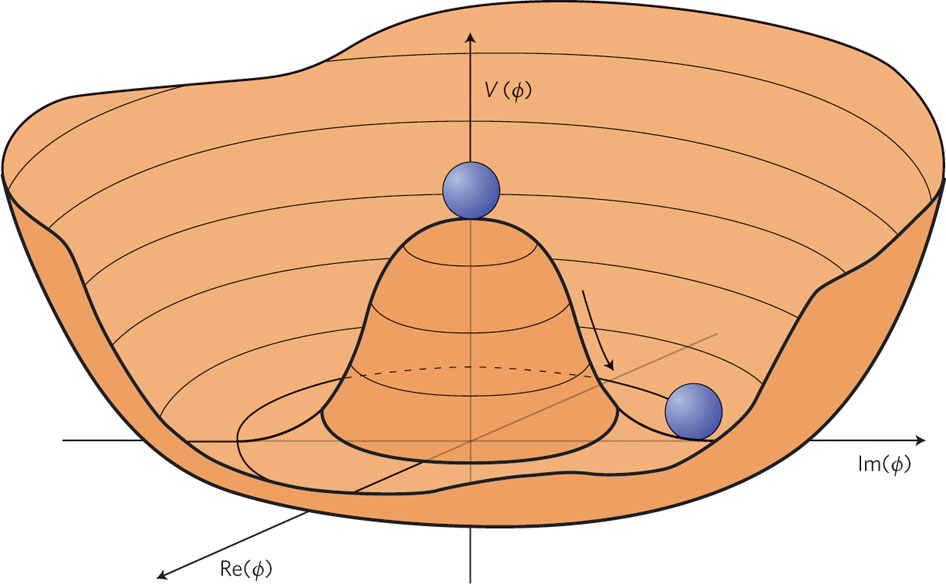
\includegraphics[width=0.6\textwidth]{Figures/Theory/MHat}
\caption{\label{fig:MexicanHat}The Higgs Potential chosen where $\mu^{2} < 0, \lambda > 0$ such that the minimum does not exist at 0, but instead in a ring of infinite minima about zero, thus introducing degeneracy and breaking the electroweak symmetry into that of QED.~\cite{MexHat}}
\end{figure}



The distinction between the two forces caused by this symmetry breaking are due to a linear combination of the weak hyper charge and isospin, $T_{3}$ and Y that vanishes for the Higgs. As this defines the conserved quantity Q for the electromagnetic group, this is not affected by the higgs, and thus the $U(1)_{em}$ group remains unbroken. Conversely, the weak portion interacts with the Higgs and the W$\pm$ and Z bosons acquire mass.  

\section{Motivation for Physics Beyond the Standard Model}
The standard model has been widely successful, predicting the existence of particles such as the $W^{\pm}$ and Z Bosons, and the t quark, showing impressive agreement with experimental findings at the level of 0.1\%. However, there are several signs that it is not a complete theory, that more information is needed to describe physics at higher energy scales. On the theoretical side, it is dissatisfying that the SM does not currently incorporate the gravitational force, explain the existence of dark matter and dark energy. Neutrino masses and flavour mixing are also unexplained, and the Higgs is as yet undiscovered. In addition, the existing SM is an effective theory, it requires several input parameters, which is seen as inelegant, as this reliance on experimental data does not reflect the fundamental picture of nature. 

The incorporation of the gravitational force has not bothered particle physicists much at the electro-weak energy scale as the strength of the effects of gravity on fundamental particles is negligible compared to the other fundamental forces. However, at an energy known as the Plank Scale, $M_{p} \sim 1-^{18}$ GeV quantum gravitational effects become important, leading to the breakdown of the existing QFT picture of the Standard Model. Thus new physics must exist at this energy scale, or before, indicating the SM is only valid up to some unknown energy scale. We think of the SM as a low-energy approximation of some larger more fundamental theory. One other fundamental problem, the hierarchy problem, shows that between the electroweak and the plank scales there lies theoretical dissatisfaction with the SM. 

As there is both theoretical and experimental concerns over the SM, this provokes theories Beyond the Standard Model (BSM), many of which come in to play at the TeV scale, which we are able to explore for the first time with the LHC. A detailed description of a few of the most interesting shortcomings most relevant to this thesis is given below.


 

\subsection{The Hierarchy Problem}
Although the Higgs Boson has yet to be observed experimentally, its mechanism is necessary to the Standard Model to provide mass to the particles, and thus is considered to exist unless proven otherwise. However, while it solves the SSB problem, the Higgs theory introduces theoretical issues of its own. The presence of the Higgs in the SM ensures the WW scattering amplitude does not violate unitarity, but only whilst the $m_{H} < 1 TeV$, providing an upper bound on the expected mass\cite{WWHMass}. 

However, in the coupling of the Higgs to heavy fermions, the mass of the Higgs receives extremely large radiative corrections. If each coupling with a fermion f has a term in the Lagrangian $-\lambda_{F} H \bar{f}f$, it contributes a quadratically divergent factor $\delta m^{2}_{H}$ that corrects the squared mass of the Higgs. 

\begin{equation}
\delta m^{2}_{H} =\sum_{f} - \frac{|\lambda_{f}|^{2}}{8 \pi^{2}}\Lambda^{2}_{UV} + \mathcal{O}(ln\Lambda)
\label{eqn:HIGGQUAD}
\end{equation}

The factor $\lambda_{f}$  represents the coupling for each type of fermion, which is largest in the case of the top quark, where $\lambda_{t} \approx 1$. The parameter $\Lambda_{UV}$ is the \textit{ultraviolet cutoff}, so named as it represents the smallest distance to probe in the calculation. It can be thought of as the scale at which the Standard Model is valid up to, as any new physics would change the theory. If there were no new physics at a lower energy, it takes the value of the Plank Scale $M_{P}$, but in this case the correction will be 30 orders of magnitude higher than the 1 TeV upper bound justified experimentally. As there exists nothing in the SM to fix the Higgs Mass, the theory requires fine-tuning, tweaking the parameters to agree with observational findings. This is generally accepted to be an inelegant method, as it requires the input of extra information, and indicates a gap in the fundamental description leading to searches for extensions to the Standard Model. 

\subsection{Cold Dark Matter}

The existence of Dark Matter was postulated as early as 1933 by Zwicky \cite{zwicky}, as the orbital velocities of galaxies in clusters were inconsistent with their observed mass, suggesting some additional mass was present but not luminous.  Measurments of rotation curves of galaxies, cosmic microwave background and structure formation have confirmed this concept over the years. Experimental results from WMAP conclude only $\sim 4.5\%$ of the energy in our universe is made of the baryonic matter we see, while dark matter accounts for $\sim 23\%$ and the rest is comprised of another unknown, dark energy~\cite{WMAP5}. Although the existence of such matter has been well documented, there is still no understanding of the physics behind the phenomena. In order to explain the properties a weakly interacting massive particle (WIMP) is required, and it must be electrically neutral. There is no provisions for such a particle in the SM, indicating additional particle content requiring extensions in the theory. 

\subsection{Unification of Coupling Constants}

At the basis of theoretical particle physics is the observation of the symmetry and simplicity of nature. Unification, where several theories can be combined into one description,  has undergone before, first Electricity and magnetism, and then electromagnetism with the weak force. While each of the three forces of the SM have their own coupling constant, as the energy scale is increased the coupling constants converge towards one another. However precision measurements show that within the current framework,  there is no common point where all three intersect. In addition, at the Planck Scale as gravity's coupling constant would be of similar strength many hope for a Grand Unified Theory (GUT),  occurring at this scale known also as the GUT scale. This is only possible with the incorporation of some new physics which would alter the trend of the couplings between the electroweak scale and this GUT scale. 


\section{Supersymmetry}

Having discussed these major issues with the SM Theory, we move on to a discussion on a potential extension to the SM. There are several options, but this thesis will focus on the theory with the best solution to the three issues highlighted discussed in detail, beginning with a natural way to eradicate the hierarchy problem simply and without fine tuning.

The hierarchy problem could be removed, rather than controlled, if there were a way to cancel out the quadratic diverging term in the Higgs mass correction. As the correction for bosons has the opposite sign, the conception of a new symmetry was born, one between fermions and bosons. Known as SUperSYmmetry (SUSY), this theory extends the SM under this symmetry such that elementary particles in the SM each have a super partner differing by one half unit of spin as yet undiscovered, just as the anti-particles were once postulated. For every fermion contributing to the quadratic divergence, a boson partner contributes the equal and opposite term, and thus the hierarchy problem cancels out and the mass of the higgs can take a sensible value.

Under this symmetry elementary particles in the SM would each have corresponding super-partners, differing by one half unit of spin, such that a fermion has a scalar boson super partner, and vice versa. At the heart of supersymmetry is a transformation that changes the field of a fermion into that of a boson, and vice versa. The generator of the transformation shall be known as Q,

\begin{equation}
\textrm{Q}|\textrm{fermion}\rangle = |\textrm{boson}\rangle,  \; \; \; \;  \textrm{Q}|\textrm{boson}\rangle = |\textrm{fermion}\rangle  
\label{eqn:Q}
\end{equation}


In addition to its neat solution to the hierarchy problem SUSY has several other consequences which lead to its position as the most favoured theory for new physics at the TeV scale. The inclusion of SUSY particles to the SM has the side affect of altering the runnings of the gauge coupling constants of the three fundamental forces, discussed above, such that they are consistent with theories of Grand Unification, an energy scale at which the three are equal. Rather than a motivation, this is a pleasant coincidence, but lends plausibility to the theory. It also shows promising features necessary for theories to incorporate gravity, although it does not finish the job. SUSY itself cannot be the final fundamental theory of particle physics, but is an extension which shows much promise, and is a pre-requisite for many higher energy theories such as most formulations of String Theory\cite{Dine}. The final, perhaps most exciting feature of SUSY is that it can offer a candidate for the particle that represents dark matter with the introduction of a new quantum number R - Parity. 



\subsection{R-Parity}

Consructing the most general form of SUSY, terms appear which allow processes which violate two quantum numbers, the baryon number B and the lepton number L. Whilst there is no theoretical reason for this to be a problem, these interactions have not been observed, and are constrained heavily. An undeniable constraint is the lifetime of the proton, which is very large, whereas these processes would facilitate its decay. whilst B and L are not fundamental symmetries in the theory, it is possible to construct a new quantum number R defined in Equation \ref{eqn:RPAR} which can be required as a symmetry R-parity. It distinguishes between particles from the SM and the sparticles introduced by SUSY, as under this construction, all SM particles carry $R$ of +1 and all super partners carry -1. 

\begin{equation}
R = (-1)^{3(B-L)+2S}
\label{eqn:RPAR}
\end{equation}
Whilst terms in the Quantum Field Theory do allow for the possibility of violation of this parity, experimental measurements has excluded this for sparticles with masses on the TeV scale, and therefore those within the reach of the LHC. Thus the  majority of searches consider models with a symmetry which forbids this violation and conserves Rp. Several phenomenological consequences that transcend specific models arise from this assumption which provide the backbone to SUSY searches at the LHC:

\begin{itemize}
\item{In order for SUSY particles to be produced at the LHC under this framework, they must be pair produced from SM particles.} 

\item{The heavier particles will cascade down a decay chain ending through creation of the lightest of the supersymmetric particles, denoted the Lightest Super Partner (LSP)}

\item{The LSP must be stable as it cannot decay into SM particles, and through cosmological bounds must be electrically neutral.} 
\end{itemize}
These characteristics of the LSP show us that it is a WIMP, the type of particle that is sought in Dark Matter searches.  These particles will not interact in a detector, therefore are characterised in an experiment as large amounts of missing energy. As this is directly a characteristic of a WIMP in the final state, such a signature represents not only SUSY but is shared by other new physics models with a dark matter candidate particle. 

Models may be constructed to constrain the violation of B and L without R-parity conservation, but those shall not be considered in this thesis, as this unique feature provides both physical motivation and a search strategy for physics at the LHC.


\subsection{MSSM} 

Whilst there are money ways to construct mathematically the theory of Supersymmery, it is usual to do it in the way which introduces the least number of new degrees of freedom. This corresponds to the minimal particle contact required to satisfy the core symmetry, which corresponds to one new degree of freedom for each existing SM one. This approach is known as the Minimal Supersymetric Standard Model (MSSM), and has an additional new particles, known as a sparticle, for each known SM particle. 

The particles are arranged to fit the irreducible representation of the symmetry, in \textit{supermultiplets}, each of which contains both fermions and bosons. The number of bosonic and fermonic degrees of freedom are therefore equal in any supermultiplet. There are two types of supermultiplet available, a chiral supermultiplet which describes a left-handed fermion, its right handed anti-particle, a complex boson and its conjugate, and a vector multiplet - a massless vector field and a left handed fermion, which result in the fermion and its anti-particle and two transversely polarised vectors bosons. 

The names of the spin-0 bosons that partner the SM fermions are prefixed with "s-", known as squarks and sleptons, collectively the sfermions. As the SM contains a distinction between left and right handed fermions, the boson super partners have one of each too, and are labelled RH and LH, but it is important to remember this is not a description of the super partner itself, merely a label to describe the SM particle is associated with. The particles are written with a tilde above the SM symbol so the top quark t becomes the "stop" quark, $\tilde{s}$.

The names of the fermions from the SM bosons are appended with "-ino" such as the super partners of the gluons, the gluinos. However, for the other fundamental SM bosons, identifying their superpartners is not so simple. The symmetry acts not on the results of electroweak symmetry breaking but on the fields of the $SU(2)_{L} \times U(1)_{Y}$ group. Thus there should be three Winos {W} and a Bino \~{B}. 

The Higgs receives different treatment in SUSY as from in the SM, where the scalar field gives up degrees of freedom to give mass to the vector bosons W$^{\pm}$ and Z.

In SUSY, instead two supermultiplets are required, one chiral and one vector, to give mass separately to the quarks of charge \sfrac{1}{3} and the quarks of charge \sfrac{2}{3}. Where the SM has one complex doublet, the MSSM has two complex Higgs doublets, hence the sector has 8 degrees of freedom. Three are lost to give the W and Z bosons mass in electroweak symmetry breaking, leaving five which represent five higgs boson particles: the charged higgs bosons $H^{\pm}$, and three neutral bosons h, H and A. The corresponding superparters are known as the higgsinos.  


\subsection{Supersymmetry Breaking}

In order to satisfy an exact symmetry, one would expect that each superpartner would have the same characteristics as its SM partner, including its mass. This would indicate they were within the reach of previous physics experiments, but it is clear this is not rue as there has been no experimental evidence of particles in the energy spectra previously covered by experimental research. Drawing parallels with the problem of electro-weak symmetry breaking, we say SUSY is broken by some mechanism, resulting in particles with heavier masses than their counterparts. Although the size of these masses could be theoretically anything, in order for SUSY to eliminate the hierarchy problem this breaking must occur at the Electroweak Scale, which puts an upper bound on the mass differences of ~1 TeV.  

This is known as "soft" SUSY breaking, and offers the hope of discovering this new physics at the TeV scale, as is now possible for the first time with the LHC. This involves "soft" mass terms incorporated into the Lagrangian theory that do not introduce quadratic divergences that would provide a new "hierarchy problem". However, the nature of this breaking is not known and thus it is traditional to formulate it in the theory to contain all the mass and mixing terms allowed by the underlying symmetry, which gives arbitrary masses to the sparticles. As there are many unknowns this introduces a large number of parameters (>50) to the system. Not all is lost, as SUSY is still capable of making useful predictions, however to compete the theory an understanding of the nature of SUSY breaking is really required. 

Due to electroweak symmetry and soft SUSY breaking the fermions superpartners of the $SU(2)_{L} \times U(1)_{Y}$ group are not generally the mass eigenstates. Instead the winos and bino mix with the higgsino fields to produce the mass eigenstates in two groups, the charginos $\tilde{\chi}^{\pm}_{1,2}$ and the neutralinos $\tilde{\chi}^{0}_{1,2,3,4}$


\subsection{Minimal Supergravity and the Constrained MSSM}

Even assuming a minimal particle content, the MSSM has a large number of free parameters, introduced through SUSY and Electroweak symmetry breaking, 105 more than the SM. When it comes to experimental searches, this is an unworkable number, for to examine possible behaviour of SUSY one would have to look in 105 dimensions. Thus for the purpose of making models to work with, it is desired to constrain this number in the theory. One popular GUT model is the theory of minimal SUper GRAvity, otherwise known as mSUGRA. 

The many parameters of the MSSM are in fact not all constants, but rather vary with the energy scale. Thus, to contain the model the we can assume that there is some ``hidden sector" (perhaps on the order of the $M_{P}$) which contains fields with no couplings to what is now thought of as the ``visible sector" of the MSSM. There should then be some messenger between the two, that allows supersymmetry braking to be mediated to the MSSM to provide the soft terms. One popular theory as to the nature of this messenger is that it is ``gravity mediated". 

The MSSM combined with the theory of mSUGRA is called the Constrained MSSM, or CMSSM, as the number of free parameters has been reduced to a manageable five. These factors are:

\begin{itemize}
\item{A common scalar mass $m_{0}$}
\item{A common gauging mass $m_{1/2}$}
\item{The SUSY Breaking common trilinear coupling $A_{0}$}
\item{The ratio of the vacuum expectation values of the two Higgs Fields tan $\beta$}
\item{ The sign of the Higgs parameter, sign($\mu$)}
\end{itemize} 

With this relatively small parameter space it is possible to construct models with which to construct search strategies, and allows us to exclude regions with the advent of new results. A given point in mSUGRA space defines the mass hierarchy of the squarks, gluinos, charginos and neutralinos, therefore governing the interactions that are possible, as well as the identity of the LSP. Thus in different regions the productions mechanisms can differ, however in the majority of phase space the LSP is the lightest of the neutralinos, $\tilde{\chi}^{0}_{1}$.  For convenience, mSUGRA is shown graphically in the $m_{0}$ - $m_{1/2}$ plane, for set values of the other three parameters. 

There are other theories that support mechanisms of SUSY breaking, such as Gauge-Mediated Symmetry Breaking (GMSB) and Anomaly Mediated Symmetry Breaking (AMSB) but these are not considered for the purpose of this thesis. 

\subsubsection{Current Limits on the CMSSM}

Two types of limits exist in mSUGRA space, those imposed theoretically and those that result from experimental data. Of the latter, some are contributed from cosmology, and others from particle physics. 

There are some regions of the parameter space where the masses of the particles have a hierarchy which results in the stau being the LSP. This is theoretically forbidden as the LSP certainly contributes some if not all of the dark matter in the universe, and it is known to be neutral. 

In addition, a further region is excluded whereby the relic density of the LSP is consistent with the WMAP measurement of the Dark Matter density. 

\subsection{Production Mechanisms in pp collisions}
At a proton-proton collider at TeV energies such as the LHC, as discussed before we can consider the protons as a set of patrons each carrying a fraction of the total momentum. It is these quarks and gluons that collide. At such high energies these can be from the gluons and the sea as well as the valence quarks, thus there are qq, $q\bar{q}$, qg and gg collisions to consider. With all of these the initial interaction is a strong production, as both quarks and gluons carry colour.  

Assuming SUSY exists within the reach of the LHC, indicated by the restriction imposed on the mass differences of SUSY Breaking, then from these interacting pairs large production rates of both squarks and gluinos are expected. Decays from these particles through charginos and neutralinos would result in production of the LSP, but the structure of these decays depends on the mass hierarchy of the sparticles, which is determined by the values of m$_{0}$ and m$_{1/2}$.  Thus a chosen point in this plane represents a certain set of kinematics. SUSY production in these collisions is dominated by the pair-productions $ qq \rightarrow \tilde{g} \tilde{g}, \tilde{q}\tilde{g}, \tilde{q} \tilde{q}$. The relative cross sections of these decay modes depend on the region of mSUGRA 

\begin{figure}
\centering
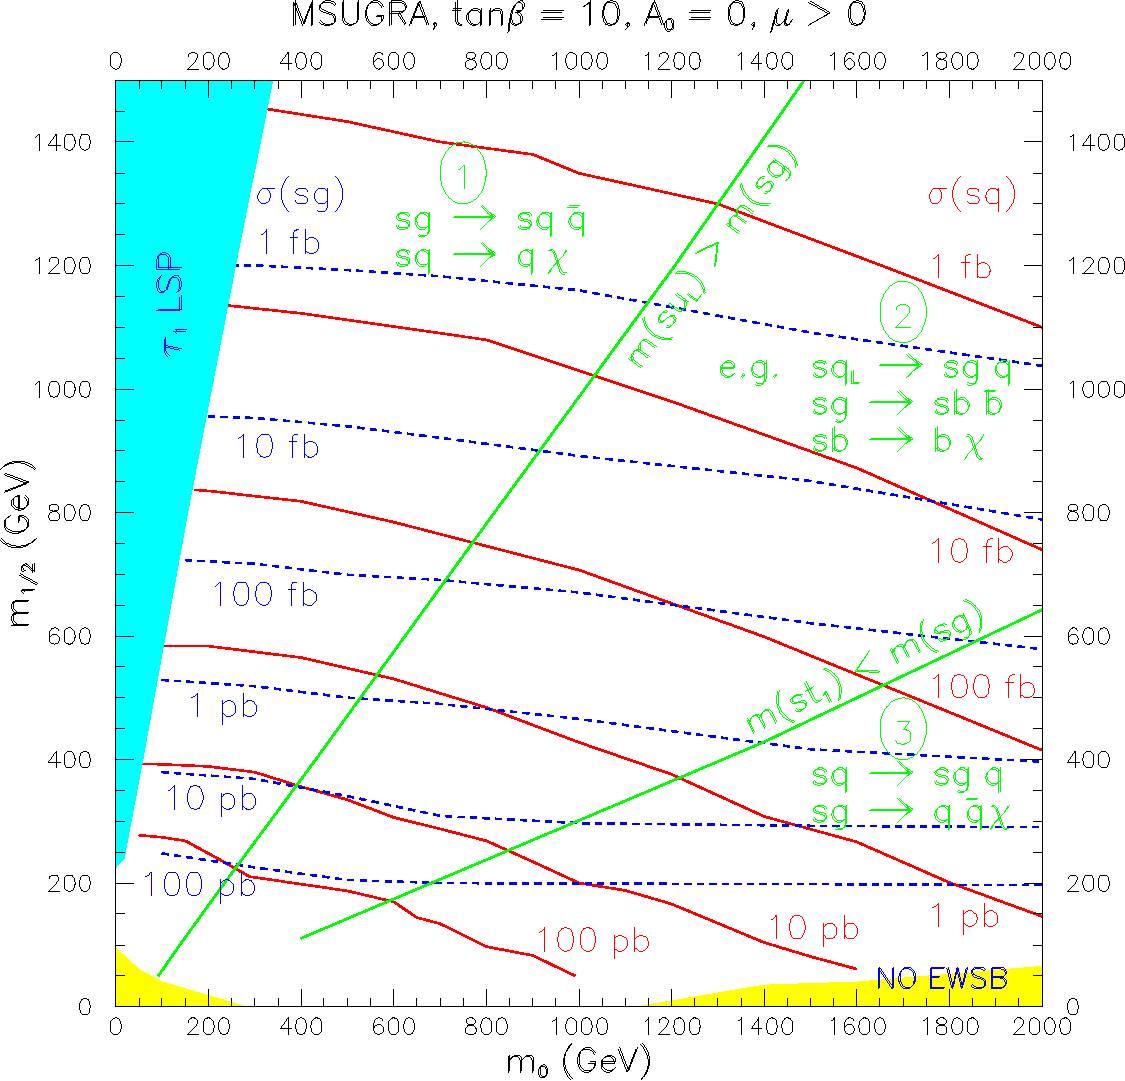
\includegraphics[width=0.6\textwidth]{Figures/Theory/mSUGRA_TDR_1}
\caption{\label{fig:msugratdr}The $m_{0}-m_{1/2}$ plane of mSUGRA depicting diagonal lines separating three distinct regions of mass hierarchies based on the mass difference of squarks and gluinos. Lines of constant production cross section for squarks and gluinos are shown in red and blue respectively. The allowed decays in each region are shown, where \textit{sq} denotes a squark, and \textit(sg) a gluino.\cite{CMSTDRII}}

\end{figure}

Within mSUGRA there are three distinct regions which exhibit different decay modes, defined by the mass relationship between the gluinos and the squarks. These an be seen Figure \ref{fig:msugratdr} , where the diagonal green lines represent a cross-over in the squark-gluino hierarchy. Passing left-right on the diagram, the regions are:

\begin{itemize}
\item{}
\item{}
\item{}
\end{itemize}





